% GNUPLOT: LaTeX picture with Postscript
\begingroup
  \makeatletter
  \providecommand\color[2][]{%
    \GenericError{(gnuplot) \space\space\space\@spaces}{%
      Package color not loaded in conjunction with
      terminal option `colourtext'%
    }{See the gnuplot documentation for explanation.%
    }{Either use 'blacktext' in gnuplot or load the package
      color.sty in LaTeX.}%
    \renewcommand\color[2][]{}%
  }%
  \providecommand\includegraphics[2][]{%
    \GenericError{(gnuplot) \space\space\space\@spaces}{%
      Package graphicx or graphics not loaded%
    }{See the gnuplot documentation for explanation.%
    }{The gnuplot epslatex terminal needs graphicx.sty or graphics.sty.}%
    \renewcommand\includegraphics[2][]{}%
  }%
  \providecommand\rotatebox[2]{#2}%
  \@ifundefined{ifGPcolor}{%
    \newif\ifGPcolor
    \GPcolortrue
  }{}%
  \@ifundefined{ifGPblacktext}{%
    \newif\ifGPblacktext
    \GPblacktexttrue
  }{}%
  % define a \g@addto@macro without @ in the name:
  \let\gplgaddtomacro\g@addto@macro
  % define empty templates for all commands taking text:
  \gdef\gplbacktext{}%
  \gdef\gplfronttext{}%
  \makeatother
  \ifGPblacktext
    % no textcolor at all
    \def\colorrgb#1{}%
    \def\colorgray#1{}%
  \else
    % gray or color?
    \ifGPcolor
      \def\colorrgb#1{\color[rgb]{#1}}%
      \def\colorgray#1{\color[gray]{#1}}%
      \expandafter\def\csname LTw\endcsname{\color{white}}%
      \expandafter\def\csname LTb\endcsname{\color{black}}%
      \expandafter\def\csname LTa\endcsname{\color{black}}%
      \expandafter\def\csname LT0\endcsname{\color[rgb]{1,0,0}}%
      \expandafter\def\csname LT1\endcsname{\color[rgb]{0,1,0}}%
      \expandafter\def\csname LT2\endcsname{\color[rgb]{0,0,1}}%
      \expandafter\def\csname LT3\endcsname{\color[rgb]{1,0,1}}%
      \expandafter\def\csname LT4\endcsname{\color[rgb]{0,1,1}}%
      \expandafter\def\csname LT5\endcsname{\color[rgb]{1,1,0}}%
      \expandafter\def\csname LT6\endcsname{\color[rgb]{0,0,0}}%
      \expandafter\def\csname LT7\endcsname{\color[rgb]{1,0.3,0}}%
      \expandafter\def\csname LT8\endcsname{\color[rgb]{0.5,0.5,0.5}}%
    \else
      % gray
      \def\colorrgb#1{\color{black}}%
      \def\colorgray#1{\color[gray]{#1}}%
      \expandafter\def\csname LTw\endcsname{\color{white}}%
      \expandafter\def\csname LTb\endcsname{\color{black}}%
      \expandafter\def\csname LTa\endcsname{\color{black}}%
      \expandafter\def\csname LT0\endcsname{\color{black}}%
      \expandafter\def\csname LT1\endcsname{\color{black}}%
      \expandafter\def\csname LT2\endcsname{\color{black}}%
      \expandafter\def\csname LT3\endcsname{\color{black}}%
      \expandafter\def\csname LT4\endcsname{\color{black}}%
      \expandafter\def\csname LT5\endcsname{\color{black}}%
      \expandafter\def\csname LT6\endcsname{\color{black}}%
      \expandafter\def\csname LT7\endcsname{\color{black}}%
      \expandafter\def\csname LT8\endcsname{\color{black}}%
    \fi
  \fi
    \setlength{\unitlength}{0.0500bp}%
    \ifx\gptboxheight\undefined%
      \newlength{\gptboxheight}%
      \newlength{\gptboxwidth}%
      \newsavebox{\gptboxtext}%
    \fi%
    \setlength{\fboxrule}{0.5pt}%
    \setlength{\fboxsep}{1pt}%
    \definecolor{tbcol}{rgb}{1,1,1}%
\begin{picture}(10800.00,7200.00)%
    \gplgaddtomacro\gplbacktext{%
      \csname LTb\endcsname%%
      \put(518,5449){\makebox(0,0)[r]{\strut{}1}}%
      \csname LTb\endcsname%%
      \put(518,5766){\makebox(0,0)[r]{\strut{}2}}%
      \csname LTb\endcsname%%
      \put(518,5951){\makebox(0,0)[r]{\strut{}3}}%
      \csname LTb\endcsname%%
      \put(518,6185){\makebox(0,0)[r]{\strut{}5}}%
      \csname LTb\endcsname%%
      \put(518,6501){\makebox(0,0)[r]{\strut{}10}}%
      \csname LTb\endcsname%%
      \put(518,6920){\makebox(0,0)[r]{\strut{}25}}%
    }%
    \gplgaddtomacro\gplfronttext{%
      \csname LTb\endcsname%%
      \put(161,6202){\rotatebox{-270}{\makebox(0,0){\strut{}Relative execution time}}}%
    }%
    \gplgaddtomacro\gplbacktext{%
      \csname LTb\endcsname%%
      \put(518,3477){\makebox(0,0)[r]{\strut{}1}}%
      \csname LTb\endcsname%%
      \put(518,3811){\makebox(0,0)[r]{\strut{}2}}%
      \csname LTb\endcsname%%
      \put(518,4007){\makebox(0,0)[r]{\strut{}3}}%
      \csname LTb\endcsname%%
      \put(518,4253){\makebox(0,0)[r]{\strut{}5}}%
      \csname LTb\endcsname%%
      \put(518,4587){\makebox(0,0)[r]{\strut{}10}}%
      \csname LTb\endcsname%%
      \put(518,5029){\makebox(0,0)[r]{\strut{}25}}%
    }%
    \gplgaddtomacro\gplfronttext{%
      \csname LTb\endcsname%%
      \put(161,4228){\rotatebox{-270}{\makebox(0,0){\strut{}Relative cycle count}}}%
    }%
    \gplgaddtomacro\gplbacktext{%
      \csname LTb\endcsname%%
      \put(616,1546){\makebox(0,0)[r]{\strut{}0.7}}%
      \csname LTb\endcsname%%
      \put(616,1855){\makebox(0,0)[r]{\strut{}1.0}}%
      \csname LTb\endcsname%%
      \put(616,2455){\makebox(0,0)[r]{\strut{}2.0}}%
      \csname LTb\endcsname%%
      \put(616,2806){\makebox(0,0)[r]{\strut{}3.0}}%
      \csname LTb\endcsname%%
      \put(616,3055){\makebox(0,0)[r]{\strut{}4.0}}%
      \csname LTb\endcsname%%
      \put(888,1448){\rotatebox{-90}{\makebox(0,0)[l]{\strut{}2mm}}}%
      \csname LTb\endcsname%%
      \put(1237,1448){\rotatebox{-90}{\makebox(0,0)[l]{\strut{}3mm}}}%
      \csname LTb\endcsname%%
      \put(1586,1448){\rotatebox{-90}{\makebox(0,0)[l]{\strut{}adi}}}%
      \csname LTb\endcsname%%
      \put(1935,1448){\rotatebox{-90}{\makebox(0,0)[l]{\strut{}atas}}}%
      \csname LTb\endcsname%%
      \put(2284,1448){\rotatebox{-90}{\makebox(0,0)[l]{\strut{}bicg}}}%
      \csname LTb\endcsname%%
      \put(2633,1448){\rotatebox{-90}{\makebox(0,0)[l]{\strut{}cholesky}}}%
      \csname LTb\endcsname%%
      \put(2982,1448){\rotatebox{-90}{\makebox(0,0)[l]{\strut{}covariance}}}%
      \csname LTb\endcsname%%
      \put(3331,1448){\rotatebox{-90}{\makebox(0,0)[l]{\strut{}doitgen}}}%
      \csname LTb\endcsname%%
      \put(3680,1448){\rotatebox{-90}{\makebox(0,0)[l]{\strut{}durbin}}}%
      \csname LTb\endcsname%%
      \put(4029,1448){\rotatebox{-90}{\makebox(0,0)[l]{\strut{}fdtd-2d}}}%
      \csname LTb\endcsname%%
      \put(4378,1448){\rotatebox{-90}{\makebox(0,0)[l]{\strut{}floyd-warshall}}}%
      \csname LTb\endcsname%%
      \put(4727,1448){\rotatebox{-90}{\makebox(0,0)[l]{\strut{}gemm}}}%
      \csname LTb\endcsname%%
      \put(5076,1448){\rotatebox{-90}{\makebox(0,0)[l]{\strut{}gemver}}}%
      \csname LTb\endcsname%%
      \put(5425,1448){\rotatebox{-90}{\makebox(0,0)[l]{\strut{}gesummv}}}%
      \csname LTb\endcsname%%
      \put(5774,1448){\rotatebox{-90}{\makebox(0,0)[l]{\strut{}heat-3d}}}%
      \csname LTb\endcsname%%
      \put(6123,1448){\rotatebox{-90}{\makebox(0,0)[l]{\strut{}jacobi-1d}}}%
      \csname LTb\endcsname%%
      \put(6472,1448){\rotatebox{-90}{\makebox(0,0)[l]{\strut{}jacobi-2d}}}%
      \csname LTb\endcsname%%
      \put(6821,1448){\rotatebox{-90}{\makebox(0,0)[l]{\strut{}lu}}}%
      \csname LTb\endcsname%%
      \put(7170,1448){\rotatebox{-90}{\makebox(0,0)[l]{\strut{}ludcmp}}}%
      \csname LTb\endcsname%%
      \put(7519,1448){\rotatebox{-90}{\makebox(0,0)[l]{\strut{}mvt}}}%
      \csname LTb\endcsname%%
      \put(7868,1448){\rotatebox{-90}{\makebox(0,0)[l]{\strut{}nussinov}}}%
      \csname LTb\endcsname%%
      \put(8217,1448){\rotatebox{-90}{\makebox(0,0)[l]{\strut{}seidel-2d}}}%
      \csname LTb\endcsname%%
      \put(8566,1448){\rotatebox{-90}{\makebox(0,0)[l]{\strut{}symm}}}%
      \csname LTb\endcsname%%
      \put(8915,1448){\rotatebox{-90}{\makebox(0,0)[l]{\strut{}syr2k}}}%
      \csname LTb\endcsname%%
      \put(9264,1448){\rotatebox{-90}{\makebox(0,0)[l]{\strut{}syrk}}}%
      \csname LTb\endcsname%%
      \put(9613,1448){\rotatebox{-90}{\makebox(0,0)[l]{\strut{}trisolv}}}%
      \csname LTb\endcsname%%
      \put(9962,1448){\rotatebox{-90}{\makebox(0,0)[l]{\strut{}trmm}}}%
      \csname LTb\endcsname%%
      \put(10311,1448){\rotatebox{-90}{\makebox(0,0)[l]{\strut{}median}}}%
    }%
    \gplgaddtomacro\gplfronttext{%
      \csname LTb\endcsname%%
      \put(161,2300){\rotatebox{-270}{\makebox(0,0){\strut{}Relative area}}}%
      \csname LTb\endcsname%%
      \put(9730,2896){\makebox(0,0)[r]{\strut{}\footnotesize Vericert-original}}%
      \csname LTb\endcsname%%
      \put(9730,2720){\makebox(0,0)[r]{\strut{}\footnotesize Vericert-list-scheduling}}%
      \csname LTb\endcsname%%
      \put(9730,2545){\makebox(0,0)[r]{\strut{}\footnotesize Vericert-hyperblock-scheduling}}%
      \csname LTb\endcsname%%
      \put(9730,2369){\makebox(0,0)[r]{\strut{}\footnotesize Bambu-no-opt}}%
    }%
    \gplbacktext
    \put(0,0){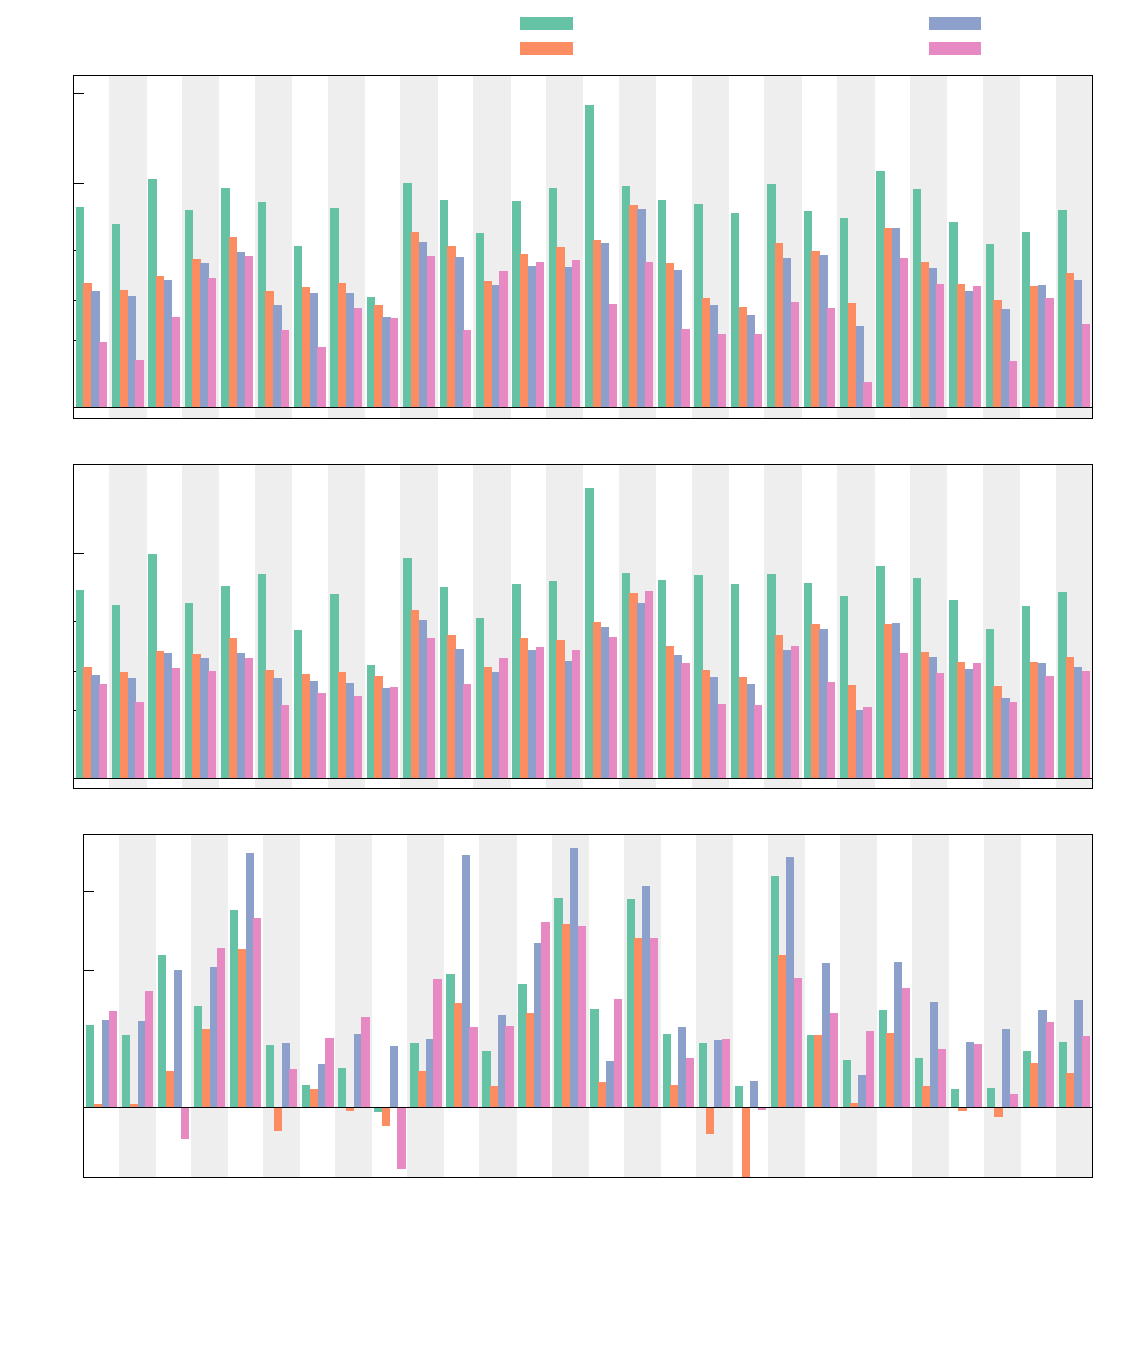
\includegraphics[width={540.00bp},height={360.00bp}]{bar-plot}}%
    \gplfronttext
  \end{picture}%
\endgroup
